\section{Utviklingsprosess}

Prosjektplanen, presentert i vedlegg \autoref{app:prosjektplan}, beskriver hvordan gjennomføringen av prosjektet opprinnelig var planlagt. Dette kapittelet bygger videre på planen og gir en redegjørelse for hvordan prosjektet faktisk ble gjennomført i praksis. Selv om den overordnede metodikken ble fulgt, ble enkelte elementer justert underveis for å tilpasse arbeidsform, fremdrift og samarbeid med eksterne aktører.

\subsection{Utviklingsmodell}
Vi valgte en smidig utviklingsmetodikk i form av scrum, med scrumboard i github projects. Videre begrunnelse og mer detaljert prosess står mer om i prosjektplanen vedlegg \autoref{app:prosjektplan}. 

\begin{figure}[H]
    \centering
    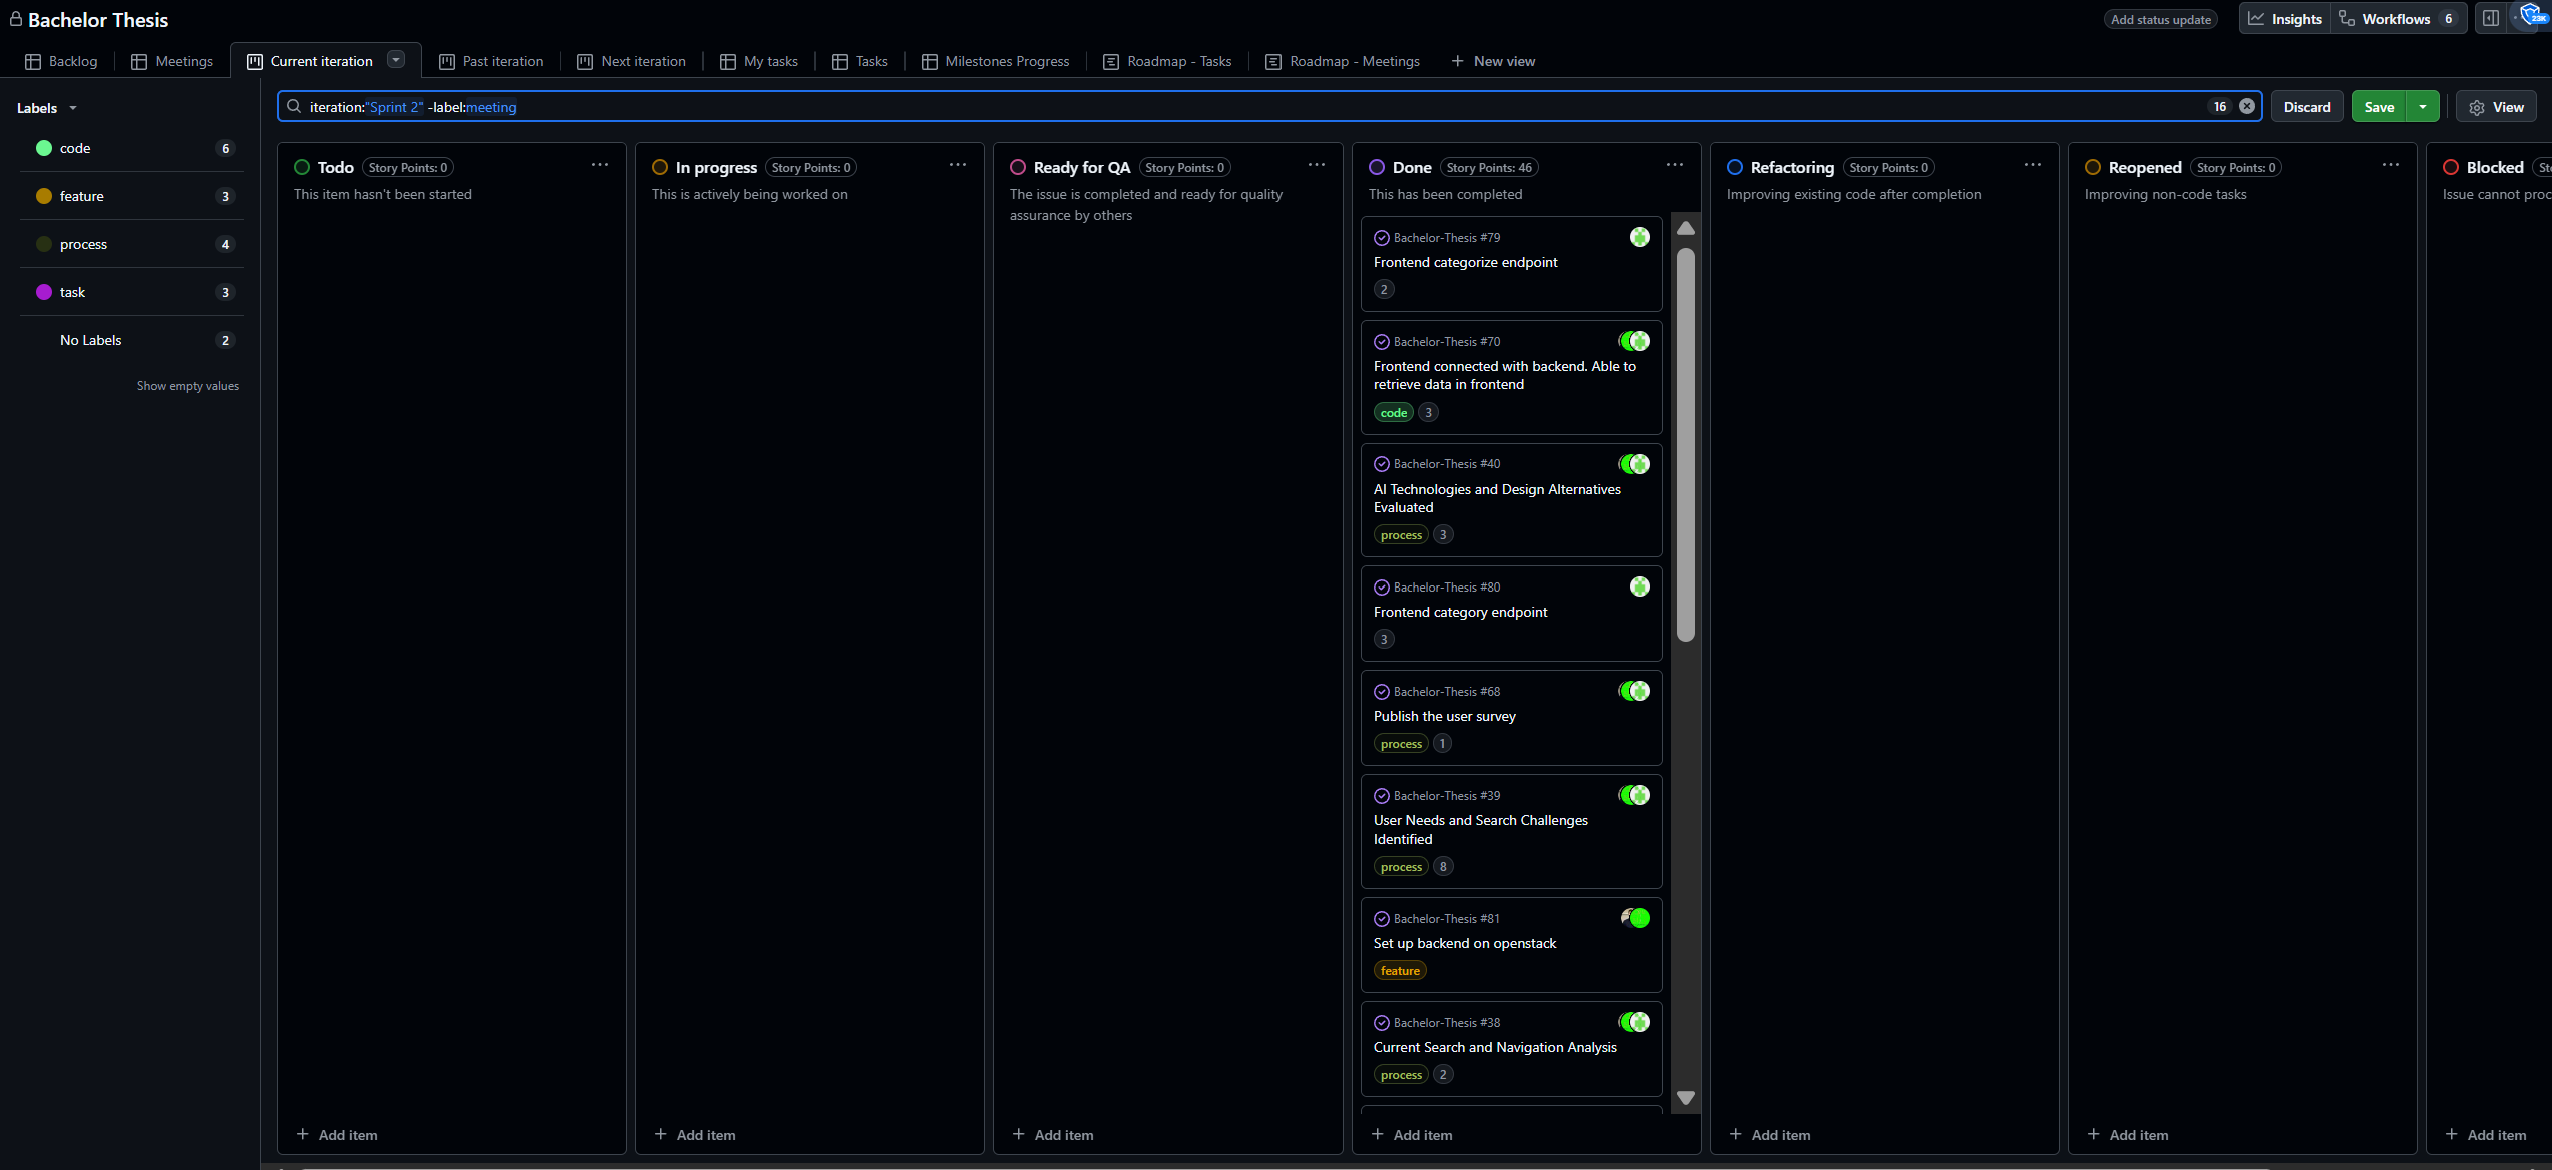
\includegraphics[width=\textwidth]{Images/ScrumBoard.png}
    \caption{Overview of the GitHub Projects scrum board  used for task tracking and sprint planning. Bildet viser hvordan en ferdig iterert sprint kan se ut (her sprint 2)}
    \label{fig:github-projects-board}
\end{figure}

\subsection{Møtestruktur og koordinering}

\subsubsection*{Daglige statusmøter}

Daglige statusmøter ble gjennomført kl. 09:15 fra mandag til fredag, primært fysisk da det var mulig. Møtene hadde kort varighet og fulgte en fast struktur hvor hvert medlem redegjorde for:

\begin{enumerate}
    \item Hva som var gjennomført siden forrige møte
    \item Hva som skulle arbeides med videre
    \item Eventuelle hindringer eller utfordringer
\end{enumerate}

Denne strukturen bidro til kontinuerlig koordinering og transparens i arbeidsprosessen. Eventuelle tekniske eller organisatoriske utfordringer ble identifisert tidlig, noe som reduserte risiko for forsinkelser og bidro til stabil fremdrift gjennom sprintene.

\subsubsection*{Sprint planlegging}
Annen hver tirsdag ble det gjennomført et sprint planleggingsmøte. Dette etterfulgte....

\subsubsection*{Veiledermøter}

Det ble gjennomført ukentlige veiledermøter hver onsdag fra kl. 12:00 til 13:00. Disse møtene hadde en mer strukturert og refleksiv karakter enn de daglige statusmøtene. Fokus lå på fremdrift i prosjektet, kvaliteten på metodiske valg, samt diskusjon av forskningsmessige utfordringer.

Veiledermøtene ble også brukt aktivt til å få tilbakemeldinger på rapportstruktur, argumentasjon og akademisk presisjon. Dette bidro til å sikre metodologisk konsistens og faglig forankring gjennom hele prosjektperioden, samtidig som det ga rom for kritisk refleksjon rundt både løsning og forskningsdesign.

\subsubsection*{Sprintgjennomgang}

Ved slutten av hver sprint ble det gjennomført sprintgjennomgang annenhver mandag kl. 10:30 sammen med Product Owner. I disse møtene ble ferdigstilt funksjonalitet demonstrert og vurdert opp mot definerte sprintmål.

I tillegg til selve demonstrasjonen ble det diskutert teknologiske løsninger, metodiske valg og arkitektoniske vurderinger. Det ble gjort sammenligninger mellom prosjektets tilnærming og Helsedirektoratets egne systemer og pågående initiativer. Dette bidro til å holde prosjektgruppen oppdatert på relevante interne føringer og teknologiske rammebetingelser hos oppdragsgiver.

Sprintgjennomgangene fungerte dermed ikke kun som en kontrollmekanisme for fremdrift, men også som en faglig dialogarena. Gjennom disse møtene fikk gruppen verdifulle referansepunkter for videre utvikling og spesialisering av løsningen, samt grunnlag for justering av prioriteringer i påfølgende sprint.

\subsubsection*{Sprintretrospektiv}

Etter hver sprintgjennomgang ble det gjennomført en intern sprintretrospektiv i Scrum-teamet. Formålet med retrospektivet var å evaluere samarbeidsprosesser, arbeidsflyt og effektivitet i gjennomføringen av sprinten.

Retrospektivene resulterte i konkrete forbedringstiltak, blant annet tydeligere avgrensning av sprintmål, mer presis oppgavefordeling og forbedret dokumentasjonspraksis. Denne iterative forbedringsprosessen bidro til økt modenhet i teamets arbeidsform over tid.

\subsubsection*{Utvidede demonstrasjonsmøter med Helsedirektoratet}

I tillegg til ordinære sprintgjennomganger ble det annenhver sprint arrangert en utvidet demonstrasjon med Helsedirektoratet, hvor flere interne representanter deltok, ikke kun Product Owner. Disse møtene hadde en bredere organisatorisk forankring og ga innsikt i hvordan løsningen ble oppfattet av ulike fagmiljøer.

De utvidede demonstrasjonene bidro til tverrfaglige tilbakemeldinger og styrket interessentforankringen i prosjektet. Ved å eksponere løsningen for flere perspektiver ble både tekniske og faglige implikasjoner tydeligere, noe som igjen påvirket videre prioriteringer og utviklingsretning. Dette styrket prosjektets relevans og tilpasning til faktiske behov hos oppdragsgiver.


\subsection{Gantt-diagram}

\begin{figure}[H] 
    \centering 
    \makebox[\textwidth][c]{%
        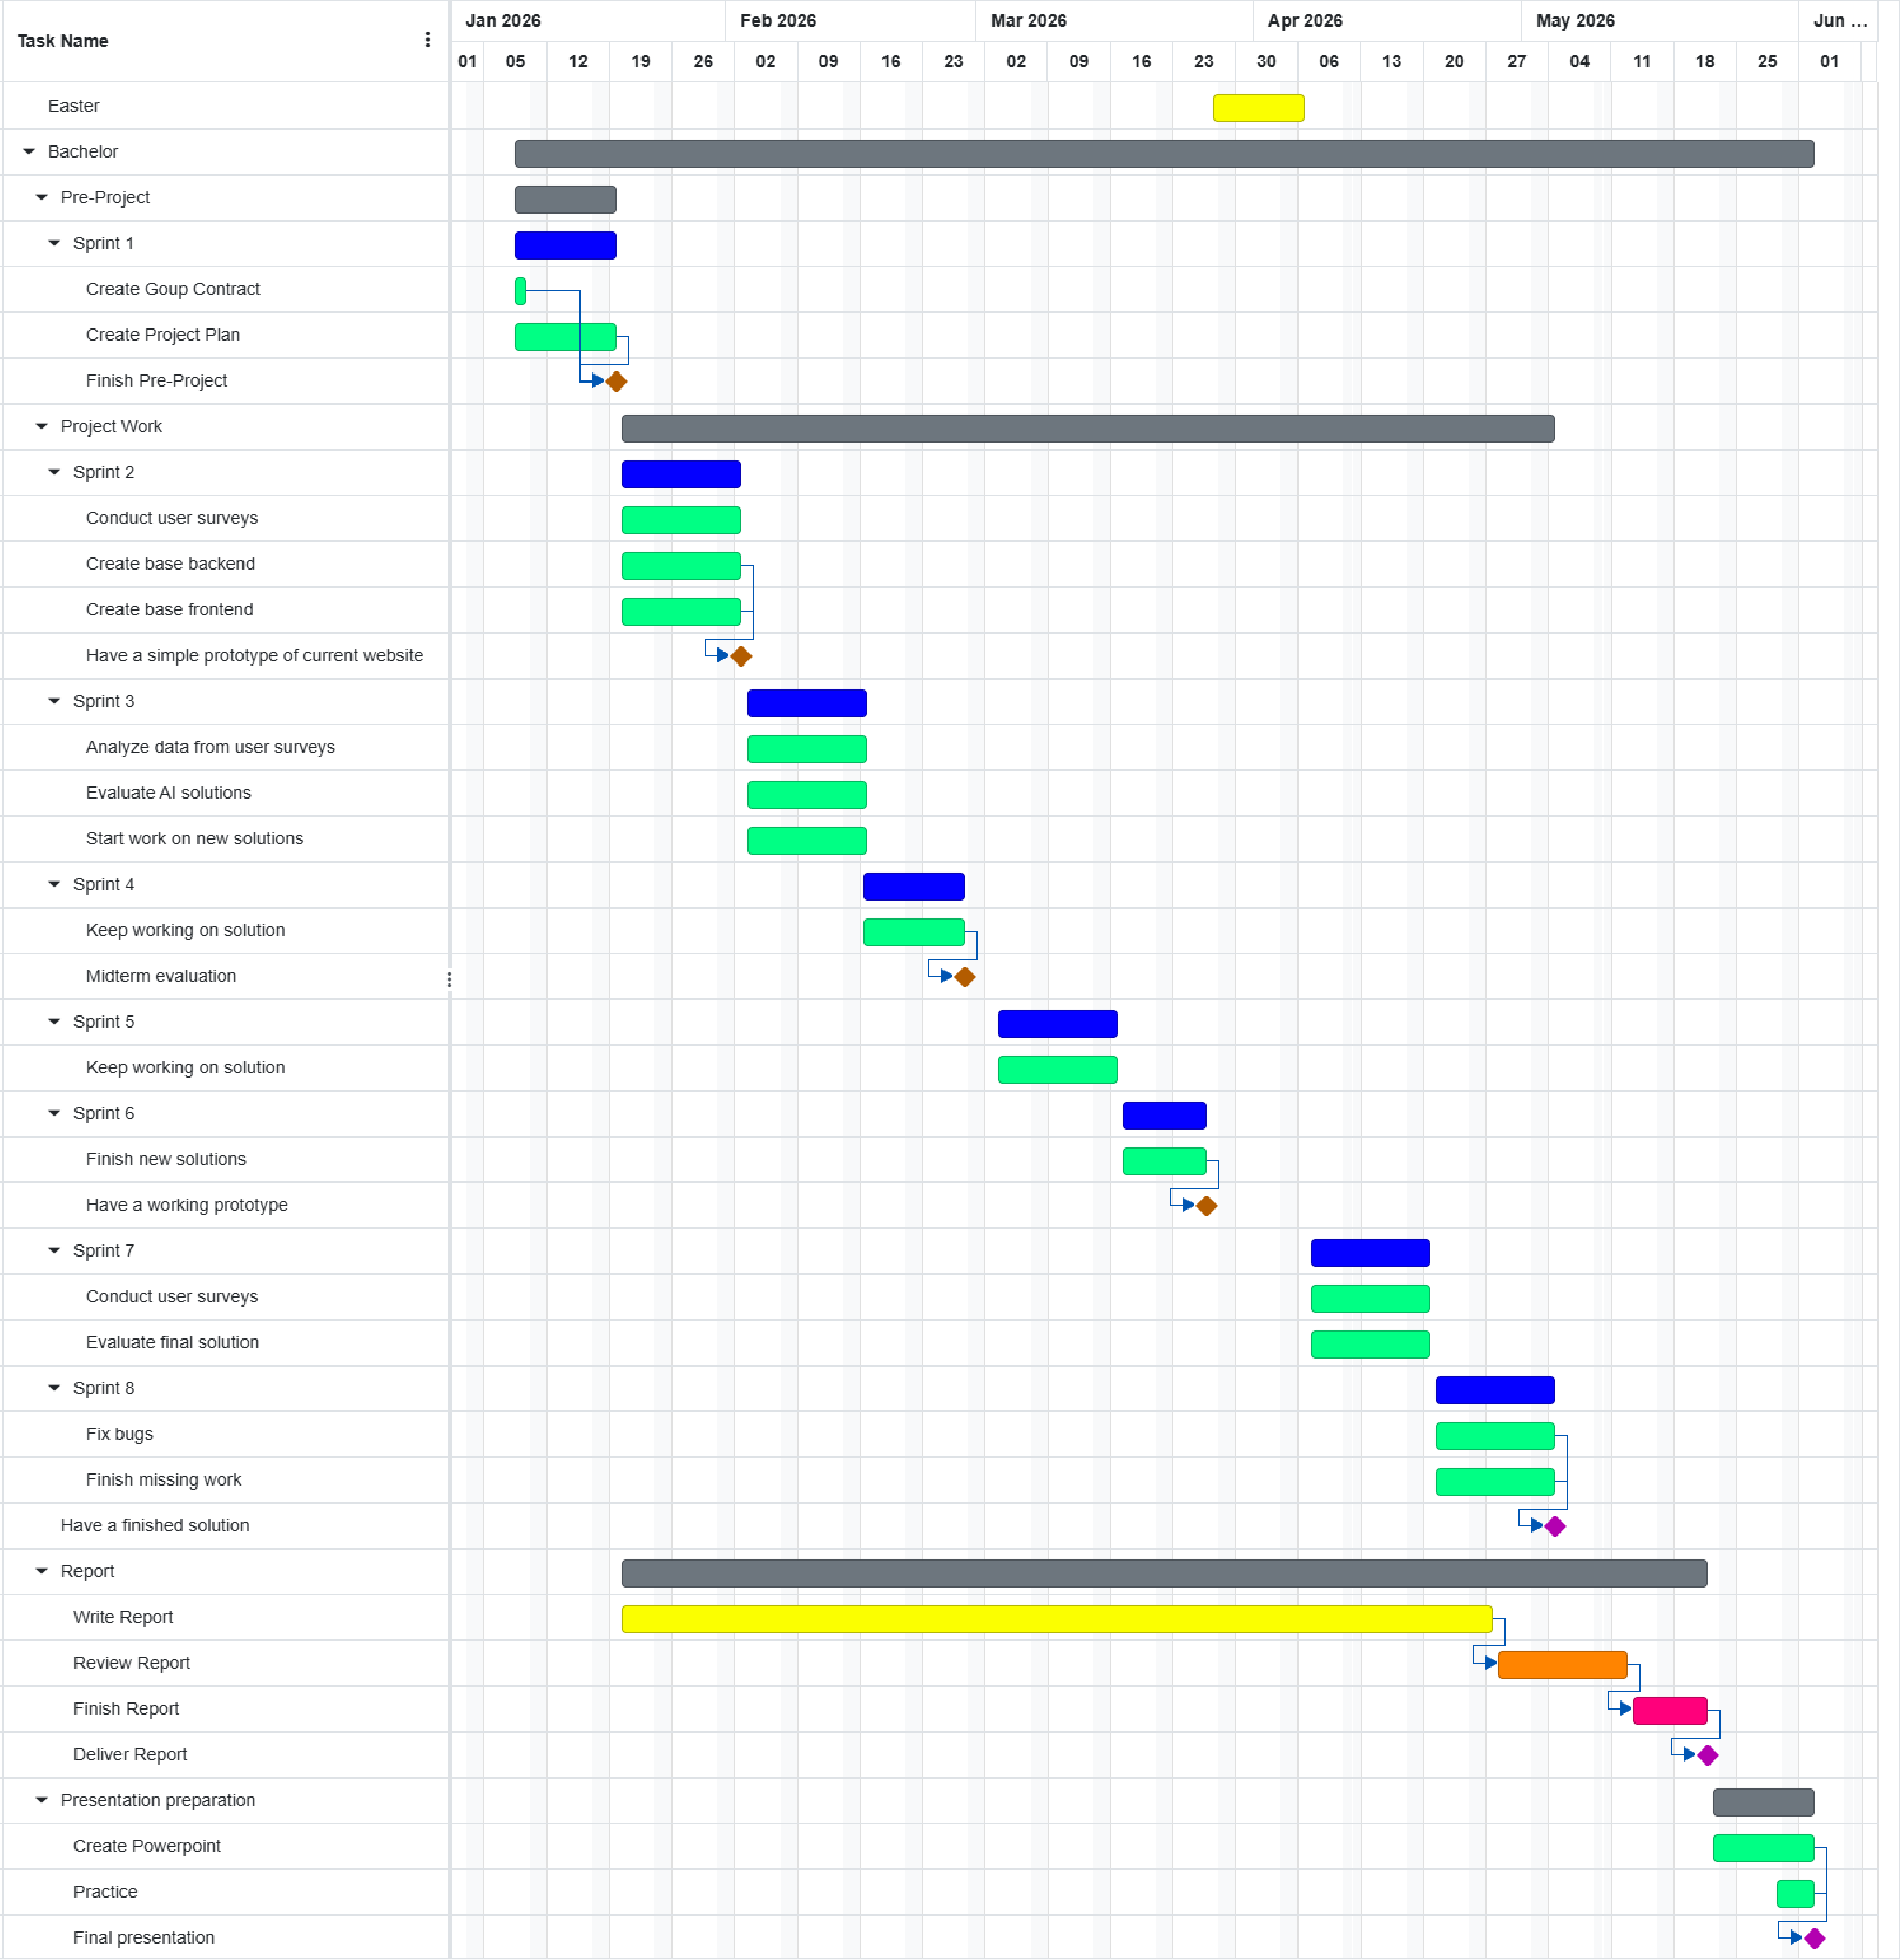
\includegraphics[width=1.2\textwidth]{Images/Gantt_diagram.pdf} 
    }
    \caption{Gantt diagram} 
    \label{fig:gantt-diagram} 
\end{figure}



\subsubsection{Gjennomføring av sprint}

\subsubsection{Sammendrag av sprinter}

\subsection*{Sprint 1 (5. jan - 19. jan)}
Starten av prosjektperioden gikk med på å lage prosjekt planen, sette opp github projects, lage gruppe kontrakt, sette opp backend, møte med helsedirektoratet og utforske deres oppsett og lage bruker undersøkelser. 

\subsection*{Sprint 2 (20. jan - 2. feb)}
Sprint to gikk ut på starte på både frotnend og backend. Det ble holdt flere møter med ansatte fra Helsedirektoratet for at gruppen skulle forstå hva som kreves for å gjøre oppgaven, der ble det konkludert med at HAPI (Helsedirektoratets API) skulle brukes til å hente innhold. Det ble satt opp en MySQL database og noe innhold ble hentet fra HAPI. Deretter ble satt opp API endpoints for søk og hetnting av innhold i backend og frontend ble koblet opp mot dette. Det ble også opprettet en brukerundersøkelse i Microsoft Forms for evaluering av Helsedirektoratets nåværende nettside. 

Det ble også gjort finpussing på prosjektplanen, slik at den kunne leveres før fristen.

\subsection*{Sprint 3 (3. feb - 16. feb)}

\subsection*{Sprint 4 (17. feb - 2. mar)}

\subsection*{Sprint 5 (3. mar - 16. mar)}

\subsection{Erfaringer og refleksjon}